\section{Modeling in SystemC}

This section explains how parts of the genetic algoritm has been modeled in SystemC and exported to hardware using HLS with Vivado. As seen in figure \ref{fig:allocation}, two components from the design can be mapped to hardware, so we constructed a SystemC model for each and tested it in the results, see section \ref{sec:results}. Both designs are made at the RTL abstraction level. This means that the communication between isolated components is abstracted away, i.e. external stimuli is simply modeled as a signal of some type and outputs are registered in a trace file. However the model is clocked, meaning we have a mean of synchronization, that is the modules are approximately timed. The two different modules will be described in the following subsections.

\subsection{GenerationGenerator}
The \textbf{GenerationGenerator} is responsible for generating a new generation of chromosomes using the generative algorithm described earlier. Using SystemC, the module consists of two SC\_CTREAD's, as it can be seen in listing \ref{lst:generationgenerator_h}. The module has a number of input and output signals, as most are self-explanatory, we will briefly review them here. The two parent inputs for generation $P_{(k)}$ stem from $P_{(k-1)}$, similar the two children of $P_{(k)}$ are parents of $P_{(k+1)}$. A chromosome has length of 64, where 32 bits are reserved for the $x$ coefficient and 32 for the $y$ coefficient of the Rosenbrock function. Mutation probability is a hyper parameter set as stimuli or from the user side. The two indecies for random numbers are used to keep track of the next random number accessed by $trueRandom()$ and created continually by $produceRandom()$.  \emph{CHR\_WIDTH} is the chromosome width.

\begin{lstlisting}[style=customc++, caption={GenerationGenerator.h},label={lst:generationgenerator_h}]
#include <systemc.h>

#define CHR_WIDTH 64
#define RANDOM_WIDTH 24
SC_MODULE(GenerationGenerator) {
  sc_in<bool> clk;
  sc_in<bool> reset;
  sc_in<bool> startGenerating;
  sc_out<bool> generatingDone;
  sc_in<sc_uint<CHR_WIDTH>> generation_parent1;
  sc_in<sc_uint<CHR_WIDTH>> generation_parent2;
  sc_out<sc_uint<CHR_WIDTH>> generation_child1;
  sc_out<sc_uint<CHR_WIDTH>> generation_child2;
  sc_in<sc_uint<RANDOM_WIDTH>> mutation_probability;
  sc_in<sc_uint<RANDOM_WIDTH>> random;
  sc_uint<RANDOM_WIDTH> randomNumberIndex;
  sc_uint<RANDOM_WIDTH> trueRandomIndex;;
  sc_uint<RANDOM_WIDTH> randomNumbers[GENERATION_SIZE * 16];

  void consumeRandom(void);
  sc_uint<RANDOM_WIDTH> produceRandom(void);
  void generateGeneration(void);
  
  SC_CTOR(GenerationGenerator) {
    randomNumberIndex = 0;
    trueRandomIndex = 0;
    SC_CTHREAD(generateGeneration, clk.pos());
    reset_signal_is(reset,false);
    SC_CTHREAD(consumeRandom, clk.pos());
    reset_signal_is(reset,false);
  }
};
\end{lstlisting}

The implementation of \textbf{GenerationGenerator} is done in SystemC. Listing \ref{lst:trueandproducerandom_cpp} shows the two functions that produce and return a random number, listing \ref{lst:generationgeneratorpragma_cpp} shows pragmas for the $generateGeneration()$ function and listing \ref{lst:generationgenerator_cpp} shows the actual implementation of the function $generateGeneration()$. Function $produceRandom()$ takes the random numbers from the input and saves them in a circular buffer. These random numbers were supposed to come from a loose audio channel, i.e. true random noise, but due to time constraints it was implemented using pseudo random numbers with the C++ $rand()$ function. Function $trueRandom()$ is used to get the random numbers when needed from the circular buffer.

\begin{lstlisting}[style=customc++,caption=The two methods for producing and accessing a random number., label={lst:trueandproducerandom_cpp}]
void GenerationGenerator::produceRandom(void) {
#pragma HLS resource core=AXI4LiteS metadata="-bus_bundle slv0" variable=random
	sc_uint<RANDOM_WIDTH> tmpRnd;
	while(true){
		randomNumbers[randomNumberIndex] = random.read();
		if(randomNumberIndex == RANDOM_WIDTH-1) {
			randomNumberIndex = 0;
		} else {
			randomNumberIndex = randomNumberIndex + 1;
		}
	}
}

sc_uint<RANDOM_WIDTH> GenerationGenerator::trueRandom(void) {
	sc_uint<RANDOM_WIDTH> randomNumber = randomNumbers[trueRandomIndex];
	if (trueRandomIndex == RANDOM_WIDTH - 1) {
		trueRandomIndex = 0; }
	else {
		trueRandomIndex = trueRandomIndex + 1;
	}
	return randomNumber;
}
\end{lstlisting}  

All signals are made available through the AXILite interface by the use of pragmas, e.g. \#pragma HLS resource core=AXI4LiteS metadata="-bus\_bundle slv0" variable=generation\_parent1, also seen in listing \ref{lst:generationgeneratorpragma_cpp}.

\begin{lstlisting}[style=customc++,caption=Pragmas defined for the GenerationGenerator function generateGeneration().,label={lst:generationgeneratorpragma_cpp}]
void GenerationGenerator::generateGeneration(void) {
  #pragma HLS resource core=AXI4LiteS metadata="-bus_bundle slv0" variable=generation_parent1
  #pragma HLS resource core=AXI4LiteS metadata="-bus_bundle slv0" variable=generation_parent2
  #pragma HLS resource core=AXI4LiteS metadata="-bus_bundle slv0" variable=generation_child1
  #pragma HLS resource core=AXI4LiteS metadata="-bus_bundle slv0" variable=generation_child2
  #pragma HLS resource core=AXI4LiteS metadata="-bus_bundle slv0" variable=generation_parent1
  #pragma HLS resource core=AXI4LiteS metadata="-bus_bundle slv0" variable=mutation_probability
  #pragma HLS resource core=AXI4LiteS metadata="-bus_bundle slv0" variable=startGenerating
  #pragma HLS resource core=AXI4LiteS metadata="-bus_bundle slv0" variable=generatingDone

  ...
\end{lstlisting}  

The $generateGeneration()$ functions contains most the logic related to generating generations. It basically implements the generative algorithm as described in theory with two random crossover points. This is done using bit masks which are AND'ed onto the parent chromosomes in the mating pool to produce new children. Each child are then mutated by a stochastic process, where a single bit in the chromosome is flipped if a given random number is lower than a scaled probability of the mutation likelihood.

\begin{lstlisting}[style=customc++,caption={GenerationGenerator.cpp},label={lst:generationgenerator_cpp}]
void GenerationGenerator::generateGeneration(void) { 
  while(true) {
    wait();	
    while (startGenerating->read() == false) { wait(); }
    generatingDone->write(false);
    sc_uint<CHR_WIDTH> parent1 = generation_parent1->read();
    sc_uint<CHR_WIDTH> parent2 = generation_parent2->read();

    // Make crossover points
    sc_uint<CHR_WIDTH> notZero = pow(2, CHR_WIDTH) - 1;
    sc_uint<RANDOM_WIDTH> point1 = trueRandom();
    sc_uint<RANDOM_WIDTH> point2 = trueRandom();

	point1 = (point1 * (CHR_WIDTH - 1)) >> RANDOM_WIDTH;
	point2 = (point2 * (CHR_WIDTH - 1)) >> RANDOM_WIDTH;
	
    // Sort high and low points
    sc_uint<RANDOM_WIDTH> highNum;
    sc_uint<RANDOM_WIDTH> lowNum;
    if(point1 > point2) {
      highNum = point1;  lowNum = point2;
    } else {
      highNum = point2; lowNum = point1;
    }
  
    sc_uint<CHR_WIDTH> bitMask1 = notZero >> lowNum & ~notZero >> highNum;
    sc_uint<CHR_WIDTH> bitMask2 = ~bitMask1;
    sc_uint<CHR_WIDTH> child1 = (parent1 & bitMask1) + (bitMask2 & parent2);
    sc_uint<CHR_WIDTH> child2 = (parent1 & bitMask2) + (bitMask1 & parent2);

    sc_uint<RANDOM_WIDTH> randomMutationProb = mutation_probability.read();

    // Mutating children
    for (int j = 0; j < CHR_WIDTH; j++) {
      if (trueRandom() < randomMutationProb) {
        child1 ^= (1 << j);
      }
      if (trueRandom() < randomMutationProb) {
      	child2 ^= (1 << j);
      }
    }
    
    generation_child1->write(child1);
    generation_child2->write(child2);
    generatingDone->write(true);
  }
}
\end{lstlisting}

The \textbf{GenerationGenerator} module is tested in a test bench that stimulates function calls to it. It simply wires the stimulation and the module together and makes a .VCD trace file with all the signals over the period of the application execution cycle, that we have included in the results. The test bench can be fount in the attached code (GenerationGenerator/main.cpp)

\subsection{Simulator}
The simulator (also called the RosenbrockSimulator in code) simulates the Rosenbrock function. The definition in SystemC can be found in listing \ref{lst:rosenbrock_h}. Function $simulateRosenbrock()$ evaluates the fitness of a chromosome from $P_{(k)}$. It should be noted that coefficients $a$ and $b$ are uint32 type signals but handled as floats in the implementation, as we were not able to successfully pass floats over the signals in SystemC. To obtain a floating value for the calculation, we simply make a type conversion using pointers. Signal \emph{chromosome\_in} is passed as input from the user side. The module outputs the actual fitness of the chromosome.

\begin{lstlisting}[style=customc++,caption={RosenbrockSimulator.h},label={lst:rosenbrock_h}]
#include <systemc.h>

#define CHROMOSOME_WIDTH 64
SC_MODULE(RosenbrockSimulator) {
  sc_in<bool> clk;
  sc_in<bool> reset;
  sc_in<bool> startSimulation;
  sc_out<bool> simulationDone;
  sc_in<sc_uint<32>> a; //actually float
  sc_in<sc_uint<32>> b; //actually float
  sc_in<sc_uint<CHR_WIDTH>> chromosome_in;
  sc_out<sc_uint<32>> fitness; //actually float

  void simulateRosenbrock(void);

  SC_CTOR(RosenbrockSimulator) {
    SC_CTHREAD(simulateRosenbrock, clk.pos());
    reset_signal_is(reset,false);
  }
};
\end{lstlisting}

The function implementation of $simulateRosenbrock()$ is viewed in listing \ref{lst:rosenbrock_cpp}. This is done using floats as an experiment, however it is not the most efficient thing to use resource-wise, but brings a better accuracy of the fitness value than fixed-point would, as the function we are looking to minimize is non-convex, i.e. multiple locally optimal points. As seen later in results in section \ref{sec:results}, we discovered there was not enough space for the module on the FPGA in terms of DSP's and LUT's. This could have been made differently by using another floating point encoding which could allow for the use of fixed point arithmetics and interpret it as floats later. $uint32ToFloat()$ is a utility function that converts a unsigned integer number to a float by a simple pointer type cast.

\begin{lstlisting}[style=customc++,caption={RosenbrockSimulator.cpp},label={lst:rosenbrock_cpp}]
#include "RosenbrockSimulator.h"
#include <string.h>
#include <math.h>
#include "ieee754float.h"

void RosenbrockSimulator::simulateRosenbrock(){
  while (true) {
    sc_uint<CHR_WIDTH> notZero = pow(2, CHR_WIDTH) - 1;
    while(startSimulation->read()==false){ wait(); }
    simulationDone->write(false);
    
    sc_uint<CHR_WIDTH> tmpChromosome = chromosome_in->read();
    sc_uint<CHR_WIDTH/2 > x = 0, y = 0;
    x = tmpChromosome >> ( CHR_WIDTH >> 1 );
    y = tmpChromosome;
    
    // Convert coefficients to floats
    float x_float = uint32ToFloat((uint32_t)x);
   	float y_float = uint32ToFloat((uint32_t)y);
   	
   	// Convert parameters to floats
   	float a_local = uint32ToFloat(a->read());
   	float b_local = uint32ToFloat(b->read());
   
   	// Evaluate Rosenbrock function with given data
    uint32_t result = pow((a_local-x_float),2)+
    		b_local*pow((y_double-pow(x_float,2)),2);
    fitness->write(result);
    simulationDone->write(true);
  }
}
\end{lstlisting}

This module is tested using a test bench in the Vivado HLS IDE. This test bench can be found in the attached code (RosenbrockSimulator/main.cpp).

\subsection{Hardware Block Design}

Lastly we view the Vivado hardware block design in figure \ref{fig:vivadodesign}. This is where we import and connect the different IP cores.
We have imported the \textbf{GenerationGenerator} RTL IP core from Vivado HLS after synthesis and wired it with an AXI interconnect component, a clock resource from the ZYNQ7 processor and a reset controller.

\begin{figure}[h!]
	\centering
	\fbox{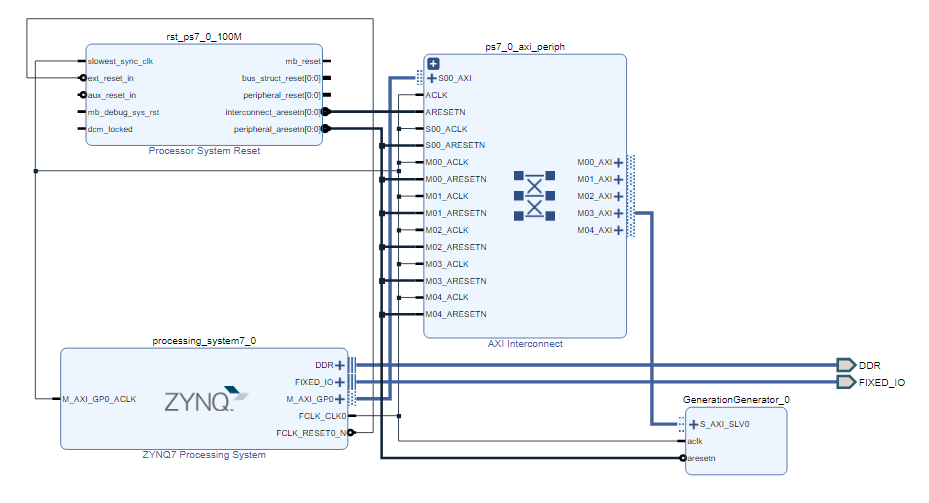
\includegraphics[width=0.7\linewidth]{../diagrams/vivadoDesign}}
	\caption{The block design in Vivado of our IP core, the ZYNQ7 processing system, a AXI interconnect component and a reset controller.}
	\label{fig:vivadodesign}
\end{figure}

Here it can be seen that we did not include all of the wanted IP cores. This was due to the Simulator using too many resources.
